% Use XeLaTeX
% Overleaf project URL : https://www.overleaf.com/project/631155904c1a625604a6ea03

\documentclass{article}

\usepackage{arxiv}

% \usepackage[french]{babel}    % Décommenter pour écrire en français
\usepackage[T1]{fontenc}      % use 8-bit T1 fonts
\usepackage{hyperref}         % hyperlinks
\usepackage{url}              % simple URL typesetting
\usepackage{booktabs}         % professional-quality tables
\usepackage{amssymb}          % blackboard math symbols
\usepackage{fontspec}         % XeLaTeX
\usepackage{nicefrac}         % compact symbols for 1/2, etc.
\usepackage{microtype}        % microtypography
\usepackage{lipsum}
\usepackage{graphicx}         % show image
\usepackage{caption}
\usepackage{subcaption}       % Figures beside each other. Requires `caption` package.
\usepackage{listings}         % Display code blocks
\usepackage{parcolumns}       % Listings beside eachother
\usepackage{xcolor}           % For listing colours

\setmainfont{Times New Roman} % XeLaTeX

\graphicspath{ {../img} }

% Reference: https://www.overleaf.com/learn/latex/Code_listing#Code_styles_and_colours
\definecolor{codegreen}{rgb}{0,0.6,0}
\definecolor{codegray}{rgb}{0.5,0.5,0.5}
\definecolor{codepurple}{rgb}{0.58,0,0.82}
\definecolor{backcolour}{rgb}{0.95,0.95,0.92}

\lstdefinestyle{pythonstyle}{
  backgroundcolor=\color{backcolour},
  commentstyle=\color{codegreen},
  keywordstyle=\color{magenta},
  numberstyle=\tiny\color{codegray},
  stringstyle=\color{codepurple},
  basicstyle=\footnotesize,
  breakatwhitespace=false,
  breaklines=true,
  captionpos=b,
  keepspaces=true,
  numbers=left,
  numbersep=5pt,
  showspaces=false,
  showstringspaces=false,
  showtabs=false,
  tabsize=4
}

\lstset{style=pythonstyle}

\title{
  Fiber Config Generator \\
  An attempt at creating a 3D white matter fiber crossing simulator using preexisting tools}


\author{
  Benoît Dubreuil \\
  Computer Science department \\
  Université du Québec à Montréal \\
  Montréal, Canada H3C 3P8 \\
  \texttt{dubreuil.benoit.2@courrier.uqam.ca} \\
  \And
  Joël Lefebvre \\
  Computer Science department\\
  Université du Québec à Montréal \\
  Montréal, Canada H3C 3P8\\
  \texttt{lefebvre.joel@uqam.ca} \\
}

\begin{document}
  \maketitle

  \begin{abstract}
    TODO: the paper abstract in 300--400 words.
  \end{abstract}


  \section{Introduction}\label{sec:introduction}

  The goal of the project Fiber Config Generator is to create a 3D white matter fiber crossing simulator to generate synthetic data in order to validate our new algorithms for processing of light sheet microscopy data~\cite{oliveirasicard2021orientation3d}.
  To do so, the project was divided into two parts: identify potential libraries to delegate the white matter phantom
  generation to and single out one according to predefined selection criteria (1), and develop an application that utilizes the selected library in order to generate high-level fiber configurations (2).
  The first part was achieved in the course ``initiation to research'' that preceded this internship, back in the winter 2022 academic term~\cite{dubreuil2022inf6200}.
  The second part is the objective of this internship, which takes place in the summer 2022 academic term~\cite{dubreuil2022inm5803simgenfork, dubreuil2022inm5803fiberconfiggen}.

  In the first part of the project, it was realized that there was an absence of fiber bundle generation-centric software.
  Consequently, non-fiber-centric software was included in the search and MRI-centric ones were the only group to come close to the project's needs~\nocite{descoteauxvalcourtcaron2022othertoolsthanfiberfox}(M. Descoteaux \& A. Valcourt Caron, virtual conversation, 21 March 2022).
  The project's requirements at that time were automation capability, ergonomics, functional independence, and being coded in Python for simplicity due to the fact that it is the main programming language used within the LINUM~\cite{dubreuil2022inf6200}.
  Thus, the library Simulation Generator was identified and then selected.

  Simulation Generator is a high-level Python API to voXSim.
  voXSim is an amelioration of Fiberfox which, contrarily to the latter, allows its users to control the white matter
  bundle generation through the command-line interface (CLI)~\cite{valcourtcaron2022simulationgenerator, neher2014fiberfox}.
  There are no Simulation Generator equivalents for Fiberfox.


  \section{Methods}\label{sec:methodology}

  GitHub was chosen as the host platform for the project's source code repository because it is free, publicly available and cloud-based, and it features free runners mainly used for DevOps practices.
  In order to be used by anyone or integrated with a bigger software, the project has to respect a minimum level of code quality.
  To do so, a continuous integration (CI) workflow was set up.
  This workflow begins with cleaning the code, then proceeds to perform a static analysis on it.

  In the static analysis workflow, a type checking pass is run.
  In order to work with external dependencies, their code must be \href{https://docs.python.org/3/library/typing.html}{type hinted}.
  Therefore, Simulation Generator was type hinted via a custom GitHub fork~\cite{dubreuil2022inm5803fiberconfiggen, valcourtcaron2022simulationgenerator}.
  It was also done to grasp the conception of that library.
  The opportunity was taken to upgrade the library's original code.
  By programming these modification, bugs were found in the original code and had to be \href{https://github.com/benoit-dubreuil/voxsim/pulls?q=is\%3Apr+is\%3Aclosed}{fixed}~\cite{dubreuil2022inm5803fiberconfiggen, valcourtcaron2022simulationgenerator}.

  Thereafter, Simulation Generator's dependencies were added to the project's dependency list (``requirements.txt'').
  Those shared with Linumpy~\cite{linum2022linumpy}, a library developed by the LINUM, were updated to the latest version.
  The listing of dependencies was patched as some were uninstallable out of the box because their compiler versions were not directly supported by the used Ubuntu versions (20.04 LTS and 22.04 LTS).

  Afterwards, Simulation Generator's significant fiber bundle geometry parameters were encapsulated into new data classes in the project.
  As the parameters were better understood, some of them were extracted as constants.

  TODO: Bugs in extracted parameters and constants, no doc to verif errors, then had to check by trial and error.
  TODO


  \section{Results}\label{sec:results}

  In the first part of the project, the software library Simulation Generator was singled out as the one that is best suited for the project's needs of automation capability, ergonomics, functional independence, and being coded in Python for simplicity due to the fact that it is the main programming language employed within the LINUM~\cite{dubreuil2022inf6200}.
  These requirements sufficed the project's goal at the time, as the LINUM team lacked firsthand experience with third-party white matter phantom simulation software.
  However, as we patched, fixed and modernized Simulation Generator through a custom GitHub fork~\cite{dubreuil2022inm5803fiberconfiggen, valcourtcaron2022simulationgenerator}, the amount of complications encountered and the required efforts to mend them increased monumentally.

  The following inadequacies were discerned:
  \begin{itemize}
    \item The source code of voXSim is inaccessible.
    \item A lot of time and efforts must be undertaken to patch, fix and adapt the library.
    These would be greatly diminished, if a CI workflow with the purpose of imposing a minimum level of code quality was implemented in the software's repository.
    \item Simulation Generator does not have any feature related to the new requirements of the project.
    \item Its strong cohesion with MITK Diffusion Fiberfox pertains to its diffusion MRI (DWI) roots.
    It is impossible to truly dissociate the brain white matter phantom from its DWI simulation, ergo a considerable amount of computer performance is wasted on this unneeded feature when generating a phantom.
    \item The generated geometric shape is unpredictable.
    Unfortunately, through trial and error, generating a simple V-shaped bundle with three anchors seems impossible.
    See the Figure~\ref{fig:f1-a} and its code Listing~\ref{lst:l1-a}.
    It is possible to generate a simple V-shaped bundle with more than three anchors.
    However, as seen in Figure~\ref{fig:f1-b} and its code Listing~\ref{lst:l1-b}, the anchors spatial positions offer next to no control over the actual shape of the resulting bundle.
    \item There is a lack of important documented features.
    Simulation Generator does not offer a possibility to modify the tension, bias and continuity of the centroid, contrarily to the description on the concepts documentation page~\cite{valcourtcaron2022simulationgenerator}.
    Although there is a piece of code about those crucial features, it is related to the XML persistence of the DWI simulation.
    In that piece of code, the parameters pertaining to the said features are in effect never set, and thus there is a possibility that may not be implemented in voXSim.
  \end{itemize}

  \begin{figure}[!htb]
    \begin{subfigure}[b]{0.4\textwidth}
      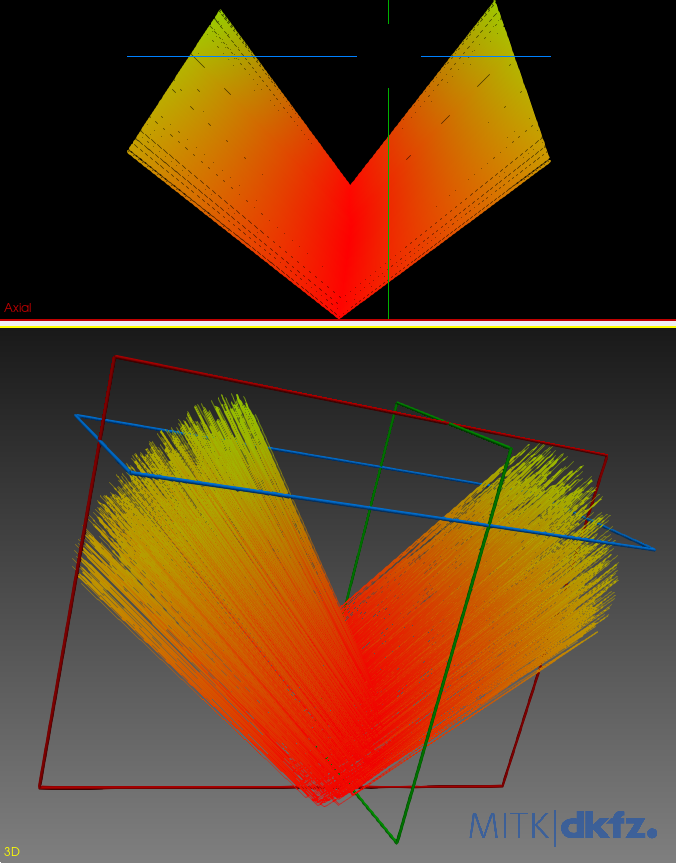
\includegraphics[width=\textwidth]{sim_gen__v_shape__good}
      \caption{Satisfactorily generated V-shaped fiber bundle}
      \label{fig:f1-a}
    \end{subfigure}
    \hfill
    \begin{subfigure}[b]{0.4\textwidth}
      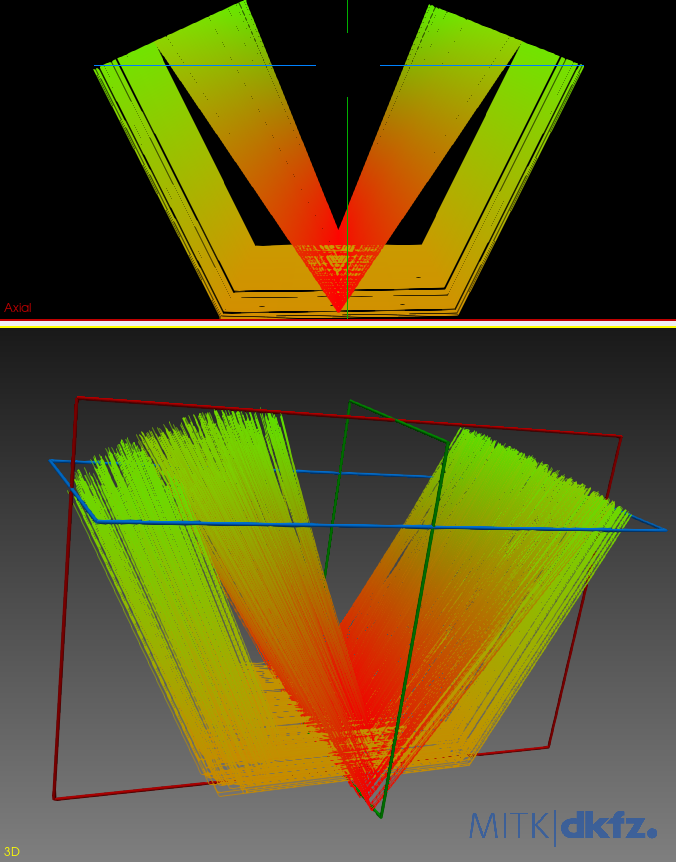
\includegraphics[width=\textwidth]{sim_gen__v_shape__bad}
      \caption{Erroneously generated V-shaped fiber bundle}
      \label{fig:f1-b}
    \end{subfigure}
    \caption{The unpredictability of Simulation Generator's fiber bundle generation. Displayed in MITK Diffusion Fiberfox~\cite{neher2014fiberfox}.}
    \label{fig:f1}
  \end{figure}

  \noindent
  \begin{minipage}[!htb]{.45\textwidth}
    % @formatter:off
    \begin{lstlisting}[language=Python, caption={Centroid anchors used to generate the fiber bundle in Figure~\ref{fig:f1-a}}, label={lst:l1-a}]
anchors = [
    (0.0, 0.0, 0.0),
    (0.25, 0.15, 0.0),
    (0.5, 0.5, 0.0),
    (0.75, 0.15, 0.0),
    (1.0, 0.0, 0.0),
]   \end{lstlisting}
    % @formatter:on
  \end{minipage}
  \hfill
  \begin{minipage}[!htb]{.45\textwidth}
    % @formatter:off
    \begin{lstlisting}[language=Python, caption={Centroid anchors used to generate the fiber bundle in Figure~\ref{fig:f1-b}}, label={lst:l1-b}]
anchors = [
    (0.0, 0.0, 0.0),
    (0.5, 0.8, 0.0),
    (1.0, 0.0, 0.0),
]   \end{lstlisting}
    % @formatter:on
  \end{minipage}

  After careful deliberation, it was decided to abandon Simulation Generator because of critical bugs, and its utility does not fit with the project's goal, especially since the main purpose of that tool is to simulate diffusion MRI (DWI) signals on generated fiber bundles.
  Simultaneously, stricter requirements and more specific to the fields of tractography and biomedical microscopy were defined.
  Thenceforth, in order to delegate the white matter phantom generation to an external library, in addition to the preceding general requirements, it is imperative that it's completely accessible and open to modifications, and that it parameterizes and allows its users to control the axon distribution and biological neural network.
  Thus, Simulation Generator is incompatible with the new sine quibus non.

  Explicitly, the new and more specific parameters are defined like so:
  \begin{itemize}
    \item \textbf{Axon distribution:} Be able to define the spatial distribution of the axons within the constrained shape of a bundle.
    By implementing a simple strategy design pattern, the default programmed distribution procedure could be, per bundle, swapped with an AI algorithm trained for a specific neuronal morphology.
    \item \textbf{Biological neural network:} Be able to subdivide individual axons into multiple paths.
  \end{itemize}


  \section{Conclusion}\label{sec:conclusion}

  In conclusion, in order to create a 3D white matter fiber crossing simulator to generate synthetic data, the usage of external MRI-centric tools with white matter generation features to circumvent the absence of fiber bundle generation-centric software~\nocite{descoteauxvalcourtcaron2022othertoolsthanfiberfox}(M. Descoteaux \& A. Valcourt Caron, virtual conversation, 21 March 2022) ought to be avoided.
  Accordingly, the development of a novel application program is recommended.
  Its requirements are of being automatable, ergonomic, functionally independent, coded in Python, open source, and parameterized at a minimum with the axon distribution, the biological neural network and the equivalent of Simulation Generator's parameters.


  \section*{Acknowledgments}\label{sec:thanks}

  I would like to thank my research professor-supervisor Joël Lefebvre who took me under his wing and trained me in the fields of image processing and neuroimaging.


  % Ajoutez vos références (format bibtex) dans le fichier references.bib
  \bibliographystyle{unsrturl}
  \bibliography{references}

\end{document}
